\documentclass[10pt]{beamer}
%\usepackage[utf8]{fontenc}
%\usepackage[utf8]{inputenc}
\usepackage[utf8]{vietnam}

%%%%%%%%%%%%%%%%%%% Bibliography %%%%%%%%%%%%%%
\usepackage{amsmath, amsthm, amssymb,latexsym,amscd,amsfonts,mathptmx,enumerate}
\usepackage[style=abntex2-alf,backend=biber,style=numeric,sorting=ynt,hyperref=auto,doi=true]{biblatex}
\addbibresource{../thesis.bib}
\usepackage{stdclsdv}
%\usepackage[unicode,hidelinks]{hyperref}

%%%%%%%%%%%%%%%%%%% Caption size %%%%%%%%%%%
%\usepackage{caption}
%\captionsetup{font=scriptsize,labelfont=scriptsize}
\setbeamerfont{caption}{size=\scriptsize}

%%%%%%%%%%%%%%%%%%% Graphics %%%%%%%%%%%%%%%
%\usepackage{chngcntr}
%\counterwithin{subfigure}{figure}
\usepackage{multicol, color, graphicx, wrapfig,afterpage,caption}
\setbeamertemplate{caption}[numbered]

\makeatletter
%%%%%%%%%%%%%%%%%%%%%%%%%%%%%% Textclass specific LaTeX commands.
 % this default might be overridden by plain title style
 \newcommand\makebeamertitle{\frame{\maketitle}}%
 % (ERT) argument for the TOC
 \AtBeginDocument{%
   \let\origtableofcontents=\tableofcontents
   \def\tableofcontents{\@ifnextchar[{\origtableofcontents}{\gobbletableofcontents}}
   \def\gobbletableofcontents#1{\origtableofcontents}
 }

%%%%%%%%%%%%%%%%%%%%%%%%%%%%%% User specified LaTeX commands.
\usetheme{Warsaw}
% or ...

\setbeamercovered{transparent}
% or whatever (possibly just delete it)

%%%%% This is for subfigure %%%%%%%%%%%%%
%\@addtoreset{subfigure}{figure}

\makeatother

%\usepackage[vietnam]{babel}

\begin{document}





\title[Khảo sát tương tác giữa phân tử protein VP35 và dsRNA của virus Ebola]{KHẢO SÁT TƯƠNG TÁC GIỮA PHÂN TỬ PROTEIN VP35 VÀ dsRNA CỦA VIRUS EBOLA}


%\subtitle{Include Only If Paper Has a Subtitle}


\author[Nguyễn Hữu Quý Ngân]{Nguyễn Hữu Quý Ngân\inst{1} \\Người hướng dẫn: TS. Nguyễn Hà Hùng Chương\inst{2}\inst{3}}


\institute[Đại học Khoa học Tự nhiên]{\inst{1}Bộ môn Vật lý Lý thuyết\\
Đại học Khoa học Tự nhiên -- ĐHQG TP.HCM\and \inst{2} Nhóm nghiên cứu Vật lý Lý thuyết, Bộ môn Khoa học Quản trị và Phát triển công nghệ\\Đại học Tôn Đức Thắng\and \inst{3} Khoa Khoa học Ứng dụng\\Đại học Tôn Đức Thắng}


\date[Tháng 7, 2015]{Báo cáo khoá luận, 2015}

\makebeamertitle


%\pgfdeclareimage[height=0.5cm]{institution-logo}{institution-logo-filename}
%\logo{\pgfuseimage{institution-logo}}



%\AtBeginSubsection[]{%
%  \frame<beamer>{ 
%    \frametitle{Tóm tắt nội dung}   
%    \tableofcontents[currentsection,currentsubsection] 
%  }
%}



%\beamerdefaultoverlayspecification{<+->}
\begin{frame}{Tóm tắt nội dung}


\tableofcontents{}




\end{frame}

\section{TỔNG QUAN}
\subsection{Bệnh gây bởi virus Ebola (EBOV)}
	\begin{frame}
	\frametitle{Bệnh gây bởi virus Ebola (EBOV)}
	
		\begin{figure}[h]
			\vspace{-20pt}
			\centering
				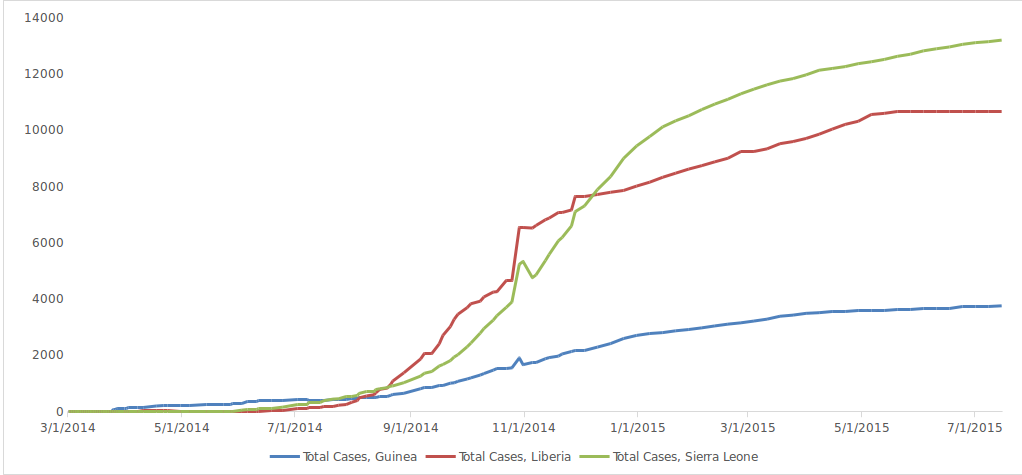
\includegraphics[height=0.5\textheight,natwidth=610,natheight=642]{numberofcases}
			\caption{Tổng số ca nhiễm bệnh tại Guinea, Liberia và Sierra Leone  \mbox{http://www.cdc.gov/vhf/ebola/outbreaks/}}
		\end{figure}
		\label{numberofcases}
		\vspace{-20pt}
		\begin{itemize}
		\item Virus Ebola (EBOV) gây nên bệnh sốt xuất huyết Ebola.
		\item Tỷ lệ tử vong khoảng 50\%, lên đến 90\%.
		\item Dơi là vật chủ trung gian.
		\end{itemize}
	\end{frame}
	
\subsection{Cơ chế hoạt động của EBOV - Phương án ngăn chặn}
	\begin{frame}
	\frametitle{Cơ chế hoạt động của EBOV - Phương án ngăn chặn}
	\begin{columns}[t]
	\begin{column}{0.5\textwidth}
		\begin{figure}[h]
		\centering
		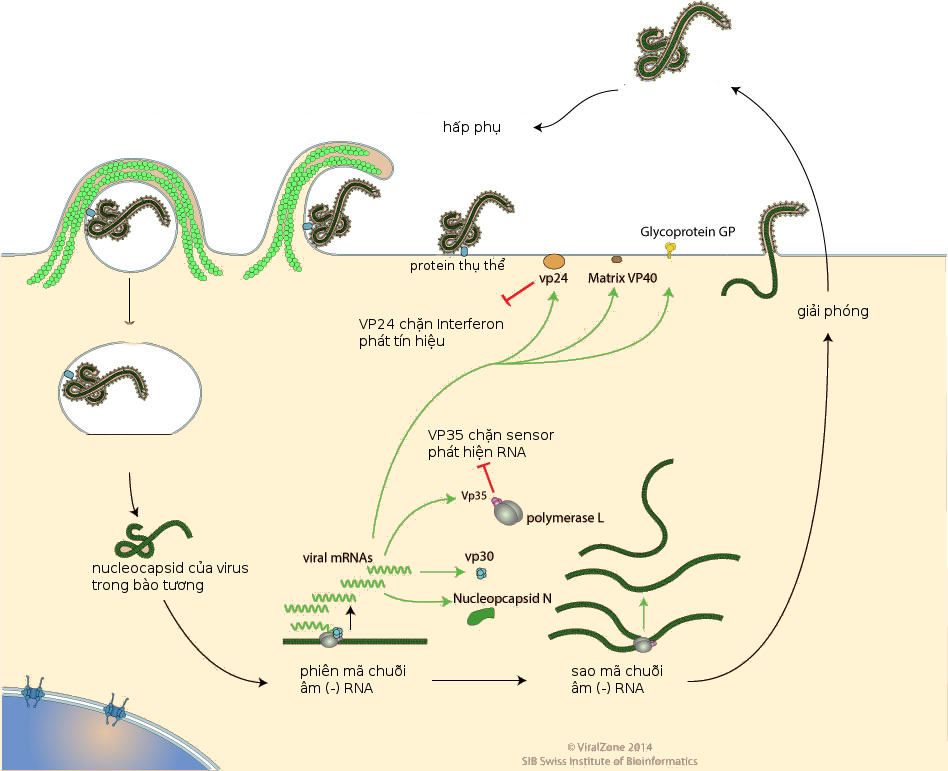
\includegraphics[height=0.5\textheight,natwidth=610,natheight=642]{../Ebolavirus_cycle.png}
		\caption{Vòng đời của EBOV: EBOV nhân lên trong bào tương và phá vỡ tế bào chui ra ngoài và gần như không bị hệ miễn dịch phát hiện. Nguồn:http://www.expasy.org/}
		\label{fig:viruscycle}
		\end{figure}
	\end{column}
	\begin{column}{0.5\textwidth}
		\begin{figure}[h]
		\centering
		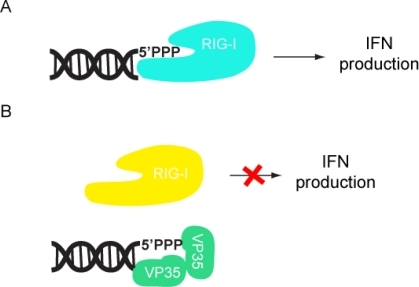
\includegraphics[height=0.25\textheight,natwidth=610,natheight=642]{../RIG-I}
		\caption{Quá trình VP35 vô hiệu RIG-I thông qua việc bám vào dsRNA. Nguồn \cite{Ramanan2011}.}
		\label{fig:rig-i}
		\vspace{-15pt}
		\end{figure}
		Ngăn chặn EBOV:
		\begin{itemize}
		\item Vaccine
		\item Tác động lên một số amino acid quan trọng của virus làm bất hoạt chức năng hoặc cản trở quá trình đóng gói virus.
		\end{itemize}
	\end{column}
	
	\end{columns}
	
	\end{frame}
\subsection{Các nghiên cứu trên thế giới về VP35}
	\begin{frame}{Các nghiên cứu trên thế giới về VP35}
		\begin{columns}[t]
		\begin{column}{0.25\textwidth}
			\begin{figure}[t!]
			\centering
			%\begin{subfigure}
			\includegraphics[width=\linewidth,natwidth=610,natheight=642]{../tongquan/1DK_3L25}
			\caption{Vị trí tương đối của ligand 1DK so với VP35 (màu xanh da trời) và dsRNA (màu vàng) đã được công bố trên \cite{Brown2014}.}
			\label{fig:1dk_3l25}
			%\end{subfigure}
			\end{figure}
		\end{column}
		
		\begin{column}{0.75\textwidth}
			\begin{enumerate}
			\item Là phân tử có tính bảo toàn cao của họ Filoviridae.
			\item Có một cấu trúc VP35 chủng Zaire Ebola (ZEBOV) nguyên thuỷ gắn với dsRNA\cite{Leung2010}.
			\item Đột biến các amino acid thứ 312, 322, 339 làm mất hoàn toàn chức năng gắn vào dsRNA của VP35\cite{Cardenas2006,Hartman2004}.
			\item Có 9 phân tử nhỏ (ligand) tương tác tốt với VP35 và tiềm năng trở thành thuốc đặc trị\cite{Brown2014,Dapiaggi2015} (xem hình \ref{fig:1dk_3l25}).				
			\item Chưa có nghiên cứu mô phỏng nào khảo sát tính chất động học của tương tác dsRNA--VP35 của virus Ebola.
			
			\end{enumerate}
			\end{column}
		\end{columns}
	\end{frame}
	
\section{ĐỐI TƯỢNG - PHƯƠNG PHÁP NGHIÊN CỨU}
\subsection{Cấu trúc 3L25 - B-conf}
	\begin{frame}
	\frametitle{Cấu trúc 3L25 - B-conf}
		\begin{columns}
			\begin{column}{0.5\textwidth}
			\begin{figure}[h]
					\centering
					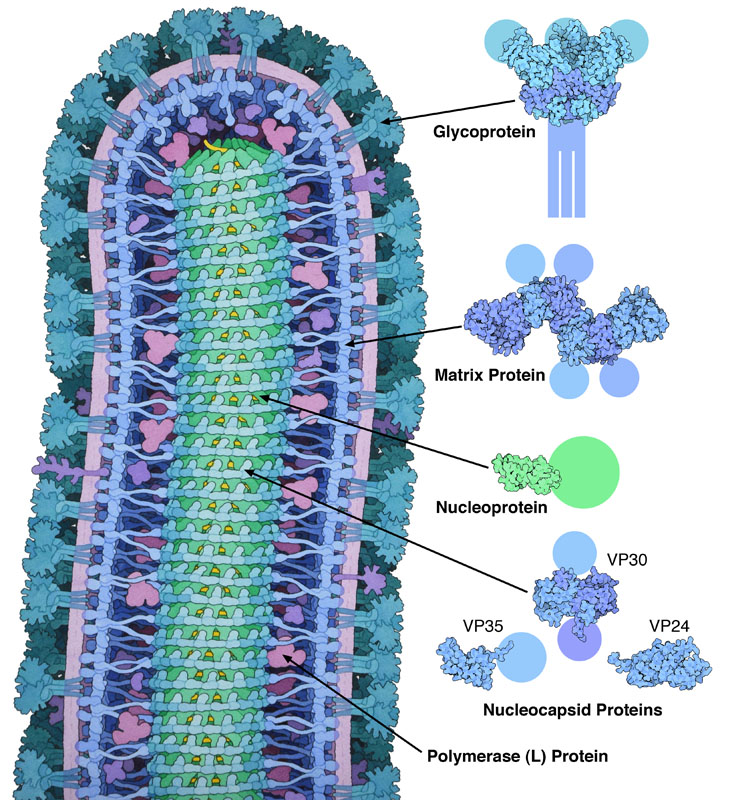
\includegraphics[height=0.6\textheight,natwidth=610,natheight=642]{../virion}
					\caption{Cấu trúc phân tử của virus Ebola \mbox{(Nguồn: www.rcsb.org)}}
			\end{figure}
			\end{column}
			\begin{column}{0.5\textwidth}
				\begin{figure}
					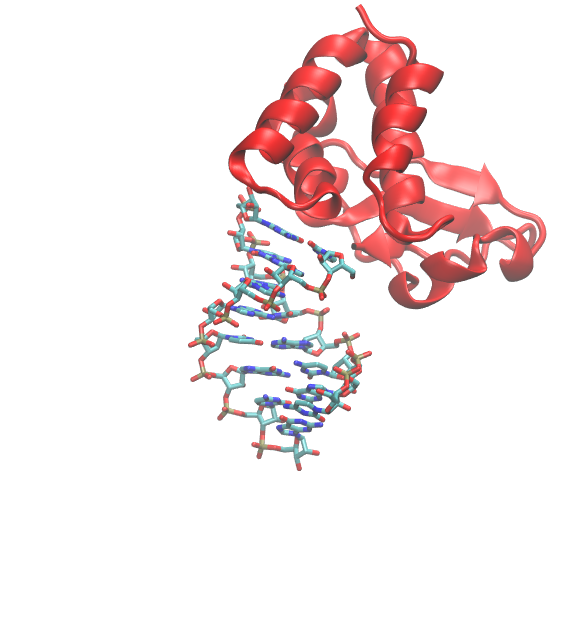
\includegraphics[height=0.6\textheight,natwidth=610,natheight=642]{../VP35_B.png}
					%\vspace{-50pt}
					\caption{Chuỗi VP35 B bám vào dsRNA dài 8bps được tô màu đỏ.}
					\label{fig:vp35b}
				\end{figure}
			
			\end{column}
		\end{columns}
	\end{frame}

\subsection{Phương pháp Mô phỏng Động học phân tử (MD)- Steered Molecular Dynamics (SMD)}
	\begin{frame}{Phương pháp Mô phỏng động học phân tử (MD)}
		\begin{wrapfigure}{r}{0.5\linewidth}
		\centering
		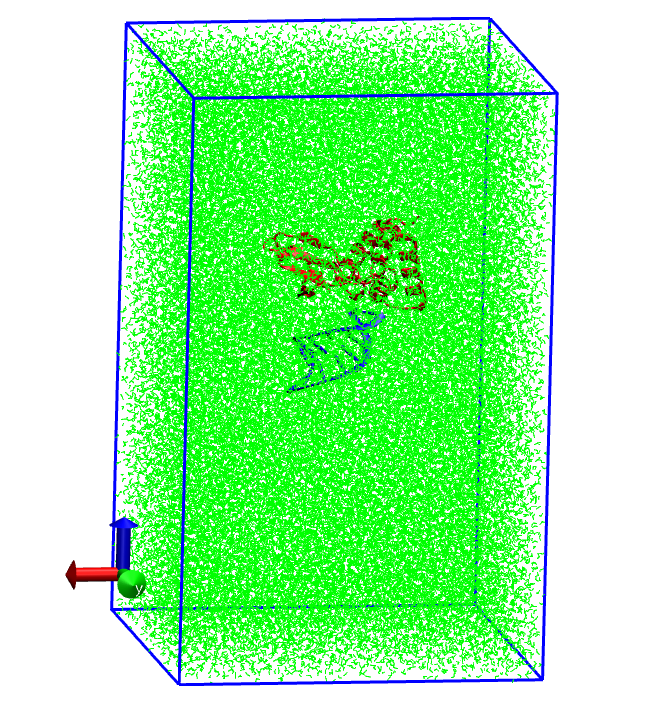
\includegraphics[width=0.7\linewidth,natwidth=610,natheight=642]{MD}
		\caption{Mô phỏng Động học phân tử - Molecular Dynamics (MD)}
		\label{fig:md}
		\end{wrapfigure}
		MD giúp khảo sát hệ nhiều hạt dựa trên phương trình chuyển động cổ điển.
		\begin{eqnarray}
		\label{force}
		\sum_{i}^{N} F_{i} = & m a_{i} \\
		\label{velocity}
		\vec{v}_{i} = & \vec{a}_{i}\cdot dt \\
		\vec{x}_{i} = & \vec{v}_{i}\cdot dt
		\label{coordinate}
		\end{eqnarray}
		%

	
		
	\end{frame}
	
	\begin{frame}{Steered Molecular Dynamics (SMD)}
		\begin{wrapfigure}{l}{0.35\linewidth}
		\vspace{-25pt}
		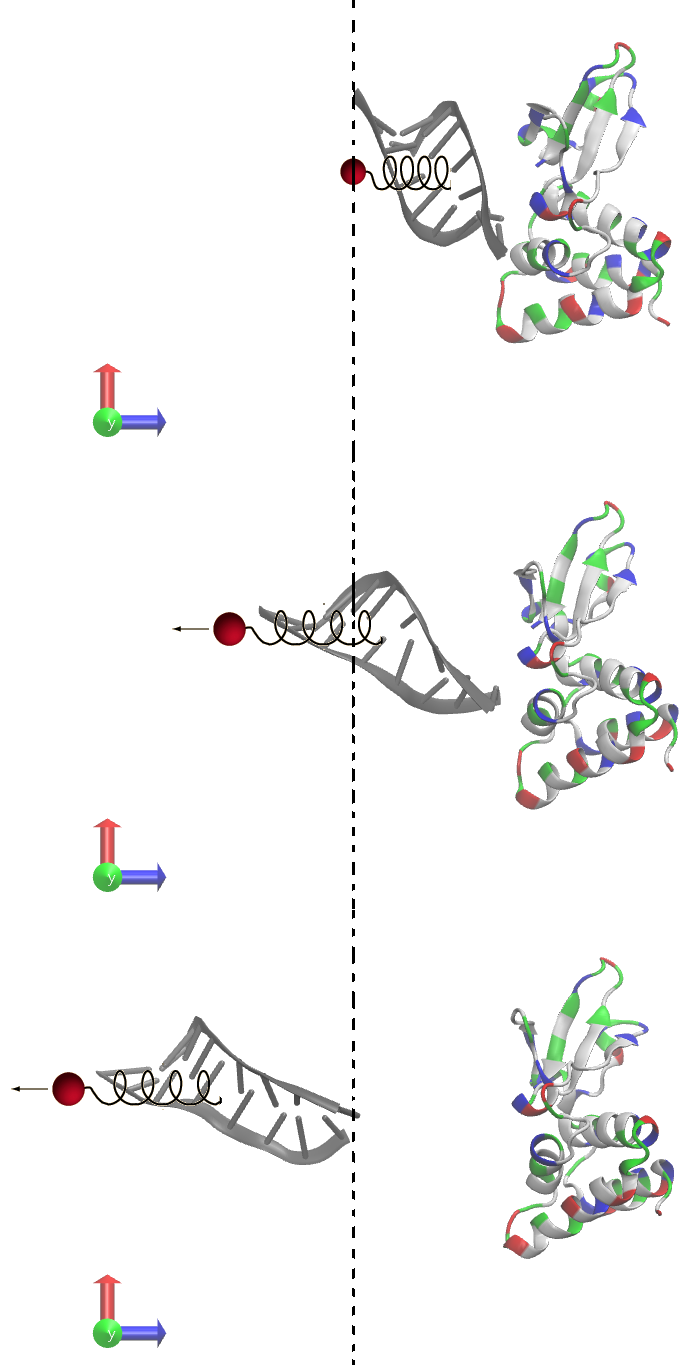
\includegraphics[height=0.7\textheight,natwidth=610,natheight=642]{../smd}
		\caption{Mô phỏng Steered Molecular Dynamics (SMD)}
		\label{fig:smd}
		\end{wrapfigure}
		SMD giúp khảo sát quá trình chuyển cấu trúc của hệ nhiều hạt bằng cách tách các nhóm phân tử ra sử dụng ngoại lực. Khoá luận sử dụng lực có thế năng dạng:
		\begin{equation}
		U_{i}\left(\vec{r}\right) = \dfrac{1}{2} k\left[ vt - \left( \vec{r}_{i}-\vec{r}_{0i} \right) \cdot\vec{n} \right]^{2}
		\end{equation}
		với $k = 1000\ \left( kJ . mol^ {-1} nm^ {-2} \right)$: hệ số đàn hồi, $v=5\left(nm/ns\right)$: tốc độ di chuyển của nhóm liên kết, $\vec{r}_{i}$: vị trí của hạt được kéo và $\vec{r}_{0i}$: vị trí ban đầu của hạt, $\vec{n}$: hướng kéo. Dưới tác dụng của thế đàn hồi, hạt sẽ chịu một lực kéo là $\vec{F}_{i} = -\vec{\nabla} U_{i} = k\left( \vec{r}_{i} - \vec{r}_{0i} -\vec{v}\times t\right)$

	\end{frame}
	
\section{KẾT QUẢ - THẢO LUẬN}
\subsection{Thiết lập hệ mô phỏng}
	\begin{frame}{Tham số sử dụng}
	\begin{columns}
	\begin{column}{0.5\textwidth}
	\begin{itemize}
	\item 193881 nguyên tử
	\item Trường lực: AMBER99SB
	\item Mô hình nước sử dụng: TIP-4P\cite{Horn2004}
	\item 3L25 (VP35 tự nhiên)
	\item 3L27 (đột biến Arg312Ala)
	\item 3L28 (đột biến Lys339Ala)
	\item VP35 đột biến Lys282Ala
	\end{itemize}
	\end{column}
	\begin{column}{0.5\textwidth}
	Các bước thiết lập:
	\begin{enumerate}
	\item Cực tiểu hóa năng lượng hệ phân tử
	\item Mô phỏng trạng thái (NVT) của hệ không đổi
	\item Mô phỏng trạng thái (NPT) của hệ không đổi
	\end{enumerate}
	\end{column}
	\end{columns}
	\end{frame}

\subsection{Thế năng của từng vị trí amino acid với dsRNA}
	\begin{frame}{Thế năng của từng vị trí amino acid với dsRNA}
		\label{fig:potential}
	\begin{columns}
	\begin{column}{0.4\textwidth}
		\begin{figure}[h]
		\centering
		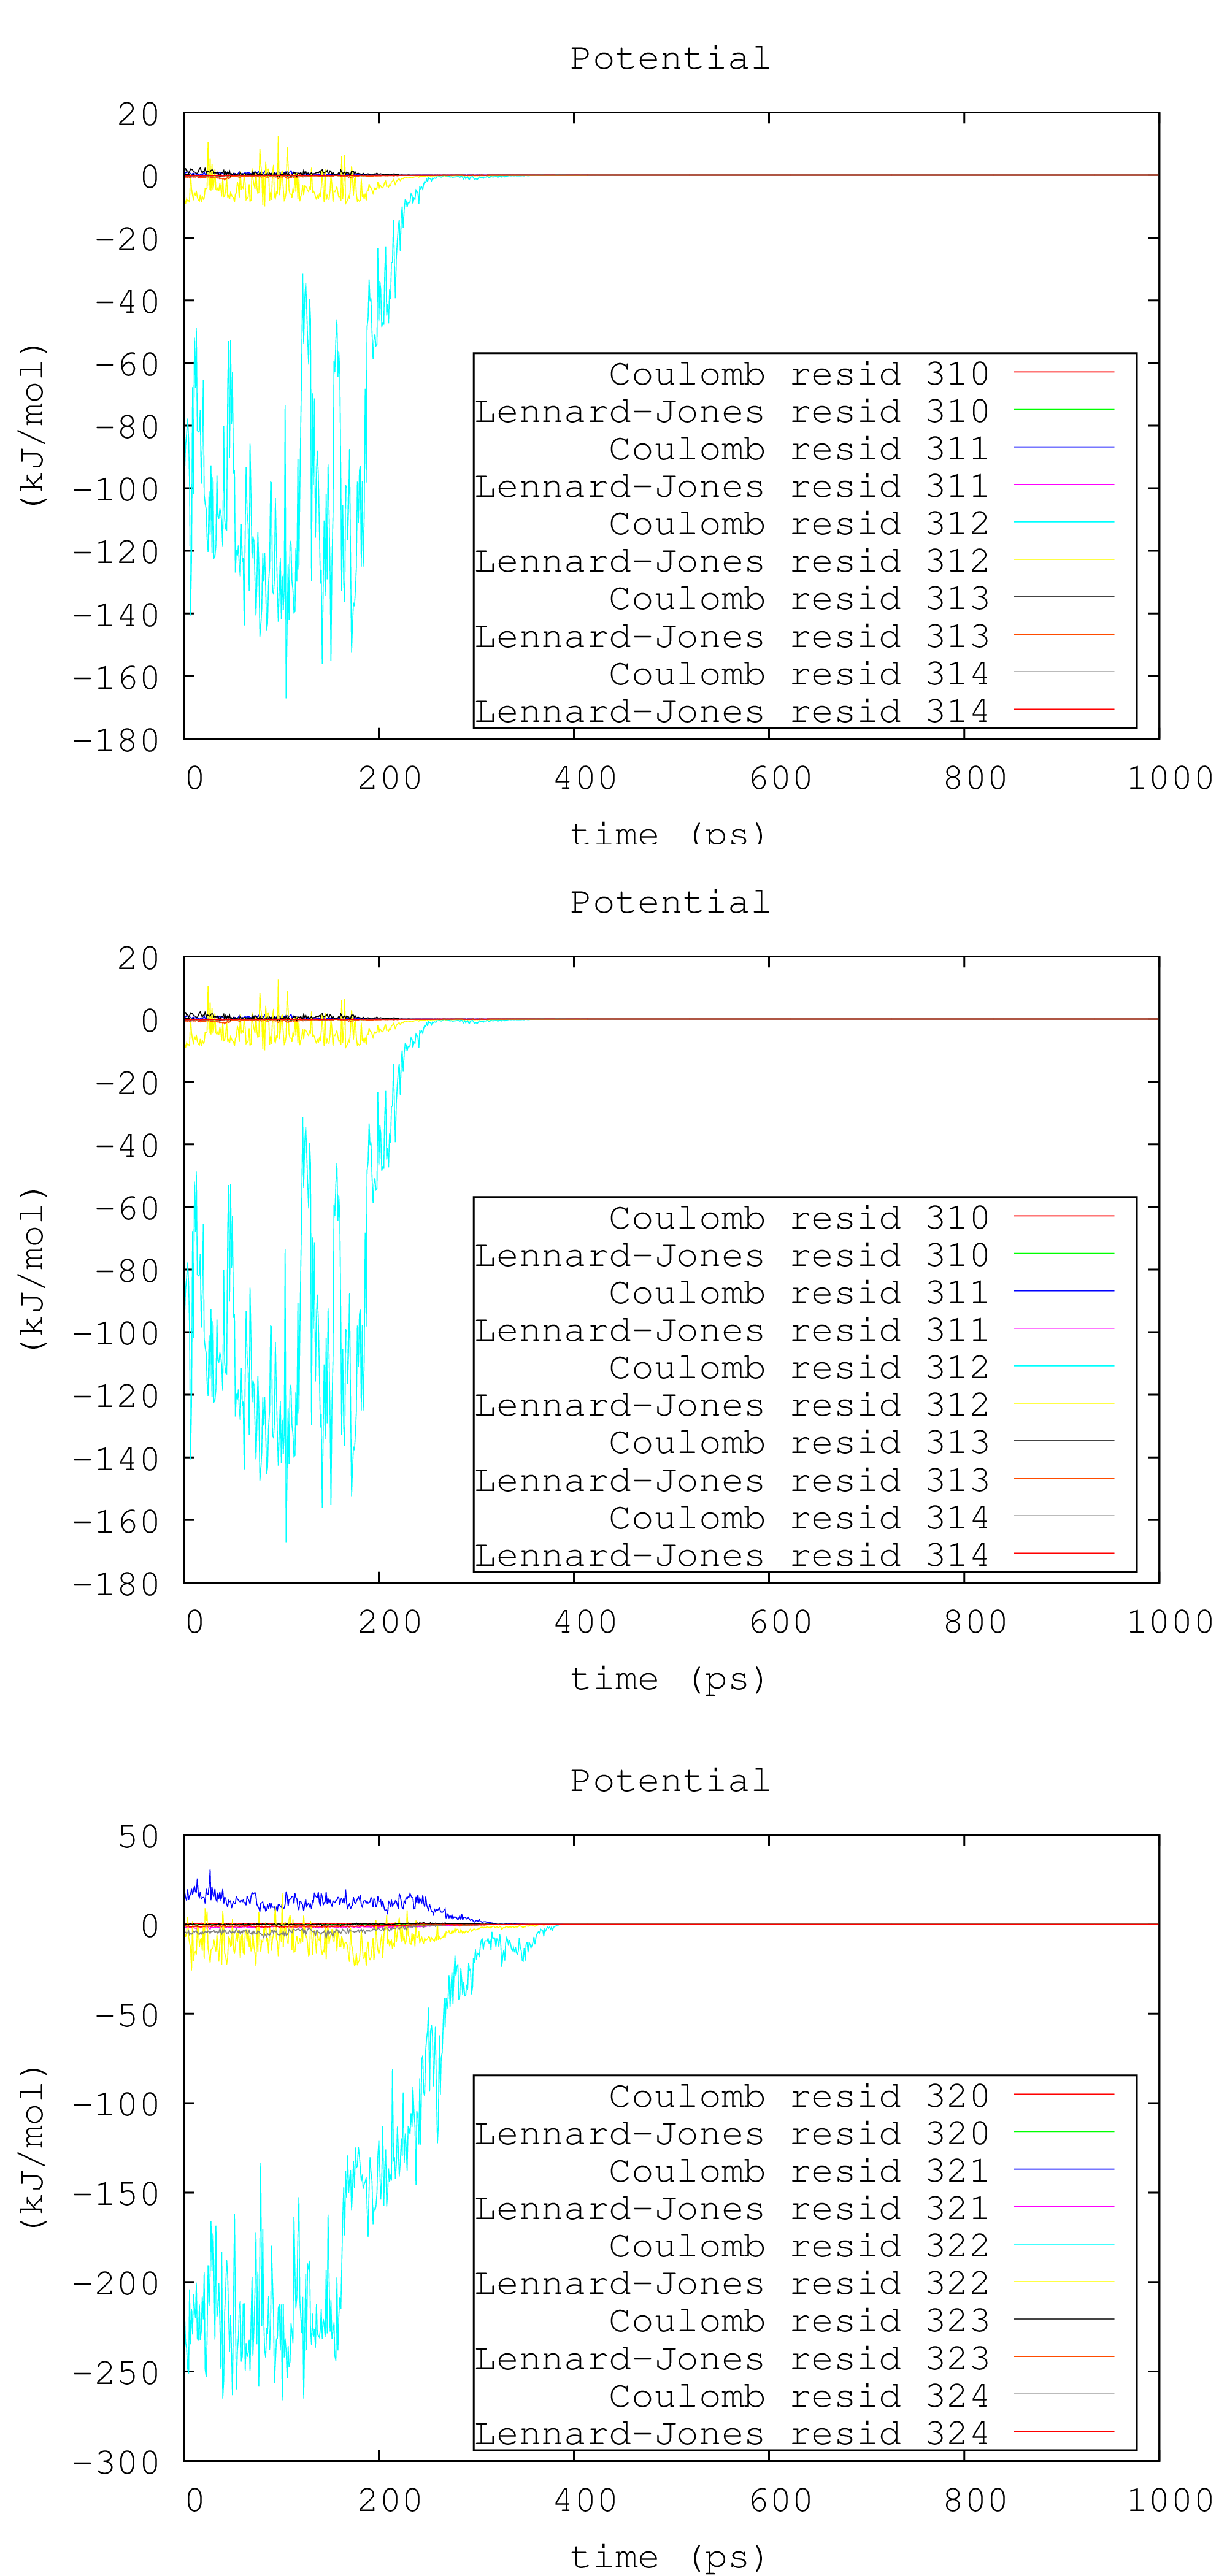
\includegraphics[height=0.7\textheight,natwidth=610,natheight=642]{potential}
		\caption{Thế năng theo thời gian của các amino acid và dsRNA.}
		\end{figure}
	\end{column}
	
	\begin{column}{0.6\textwidth}
	\begin{enumerate}
		\item Chọn ra 81 vị trí amino acid của VP35 có khả năng tương tác với dsRNA.
		\item Thế năng giữa amino acid và dsRNA thay đổi theo thời gian đặc trưng cho tương tác trực tiếp giữa amino acid đó và dsRNA.
		\item Thu được 3 vị trí amno acid có sự biến thiên thế năng lớn: Lys282, Arg312, Arg322.
	\end{enumerate}
	\end{column}
	\end{columns}
	\end{frame}


\subsection{Liên kết Hydro giữa các vị trí amino acid với dsRNA}
	\begin{frame}{Liên kết Hydro giữa các vị trí amino acid với dsRNA}
		\label{fig:hbond}
	\begin{columns}
	\begin{column}{0.5\textwidth}
		\begin{figure}[h]
		\centering
		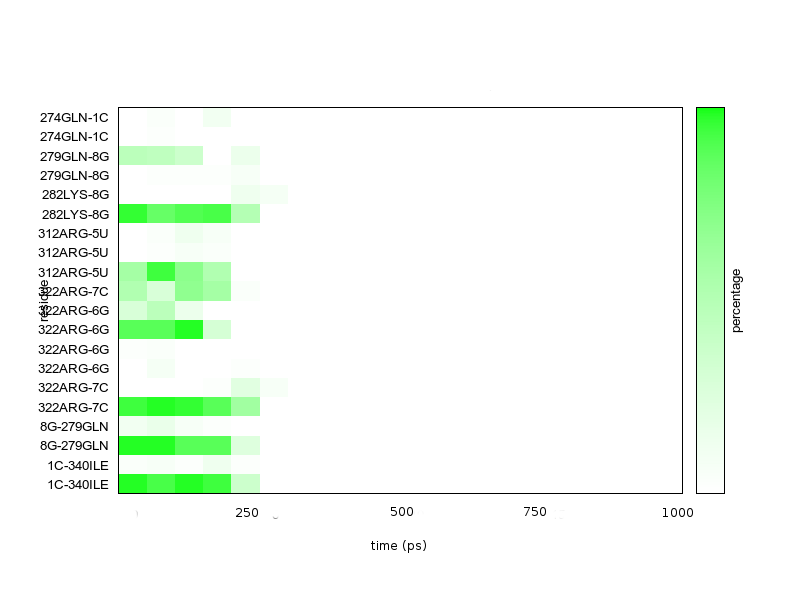
\includegraphics[width=\textwidth,natwidth=610,natheight=642]{../hbond3L25_pull2}
		\caption{Đồ thị liên kết Hydro theo thời gian giữa các vị trí amino acid và dsRNA trong lần mô phỏng SMD thứ hai.}
		\end{figure}
	\end{column}
	
	\begin{column}{0.5\textwidth}
		\begin{itemize}
		\item Trong môi trường nước, liên kết Hydro chiếm ưu thế và đóng góp nhiều cho tương tác giữa hai nhóm nguyên tử.
		\item Các vị trí amino acid tạo liên kết Hydro với dsRNA nhiều nhất: Glu279, Lys282, Arg312, Arg322, Ile340.
		\end{itemize}
	\end{column}
	\end{columns}
	\end{frame}


\subsection{Lực kéo sử dụng để tách VP35 và dsRNA}
	\begin{frame}{Tương quan giữa lực kéo tối đa và năng lượng liên kết}
	\begin{columns}
	\begin{column}{0.5\textwidth}
		\begin{figure}[t]
		\centering
		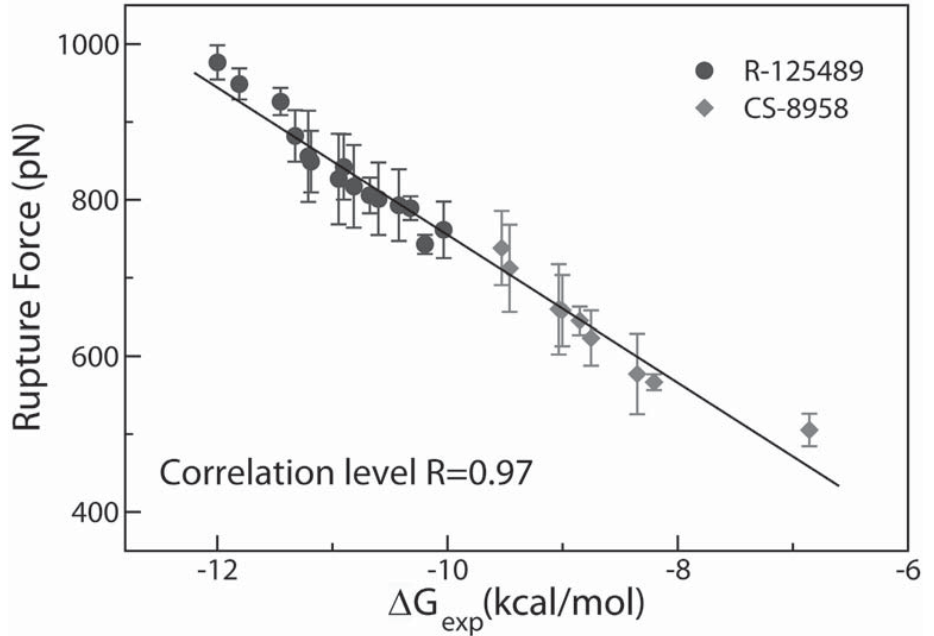
\includegraphics[width=0.7\textwidth,natwidth=610,natheight=642]{../rupture_force-delta_G}
		\caption{Đồ thị tương quan giữa lực kéo tối đa (Rupture Force) và năng lượng tương tác giữa phân tử R-125489 với thụ thể NA của virus cúm và giữa phân tử CS-8959 với thụ thể NA của virus cúm \cite{SuanLi2012}. Hệ số tương quan (correlation level) R = 0.97}
		\label{fig:rupture-force-delta-g}
		\end{figure}
	\end{column}
	
	\begin{column}{0.5\textwidth}
	\begin{itemize}
	\item Lực kéo tối đa (Rupture force) tỷ lệ với năng lượng liên kết giữa hai nhóm phân tử.
	\end{itemize}
	\end{column}
	\end{columns}
	\end{frame}
	
	\begin{frame}
	\begin{columns}
	\begin{column}{0.5\textwidth}
		\begin{figure}[t]
		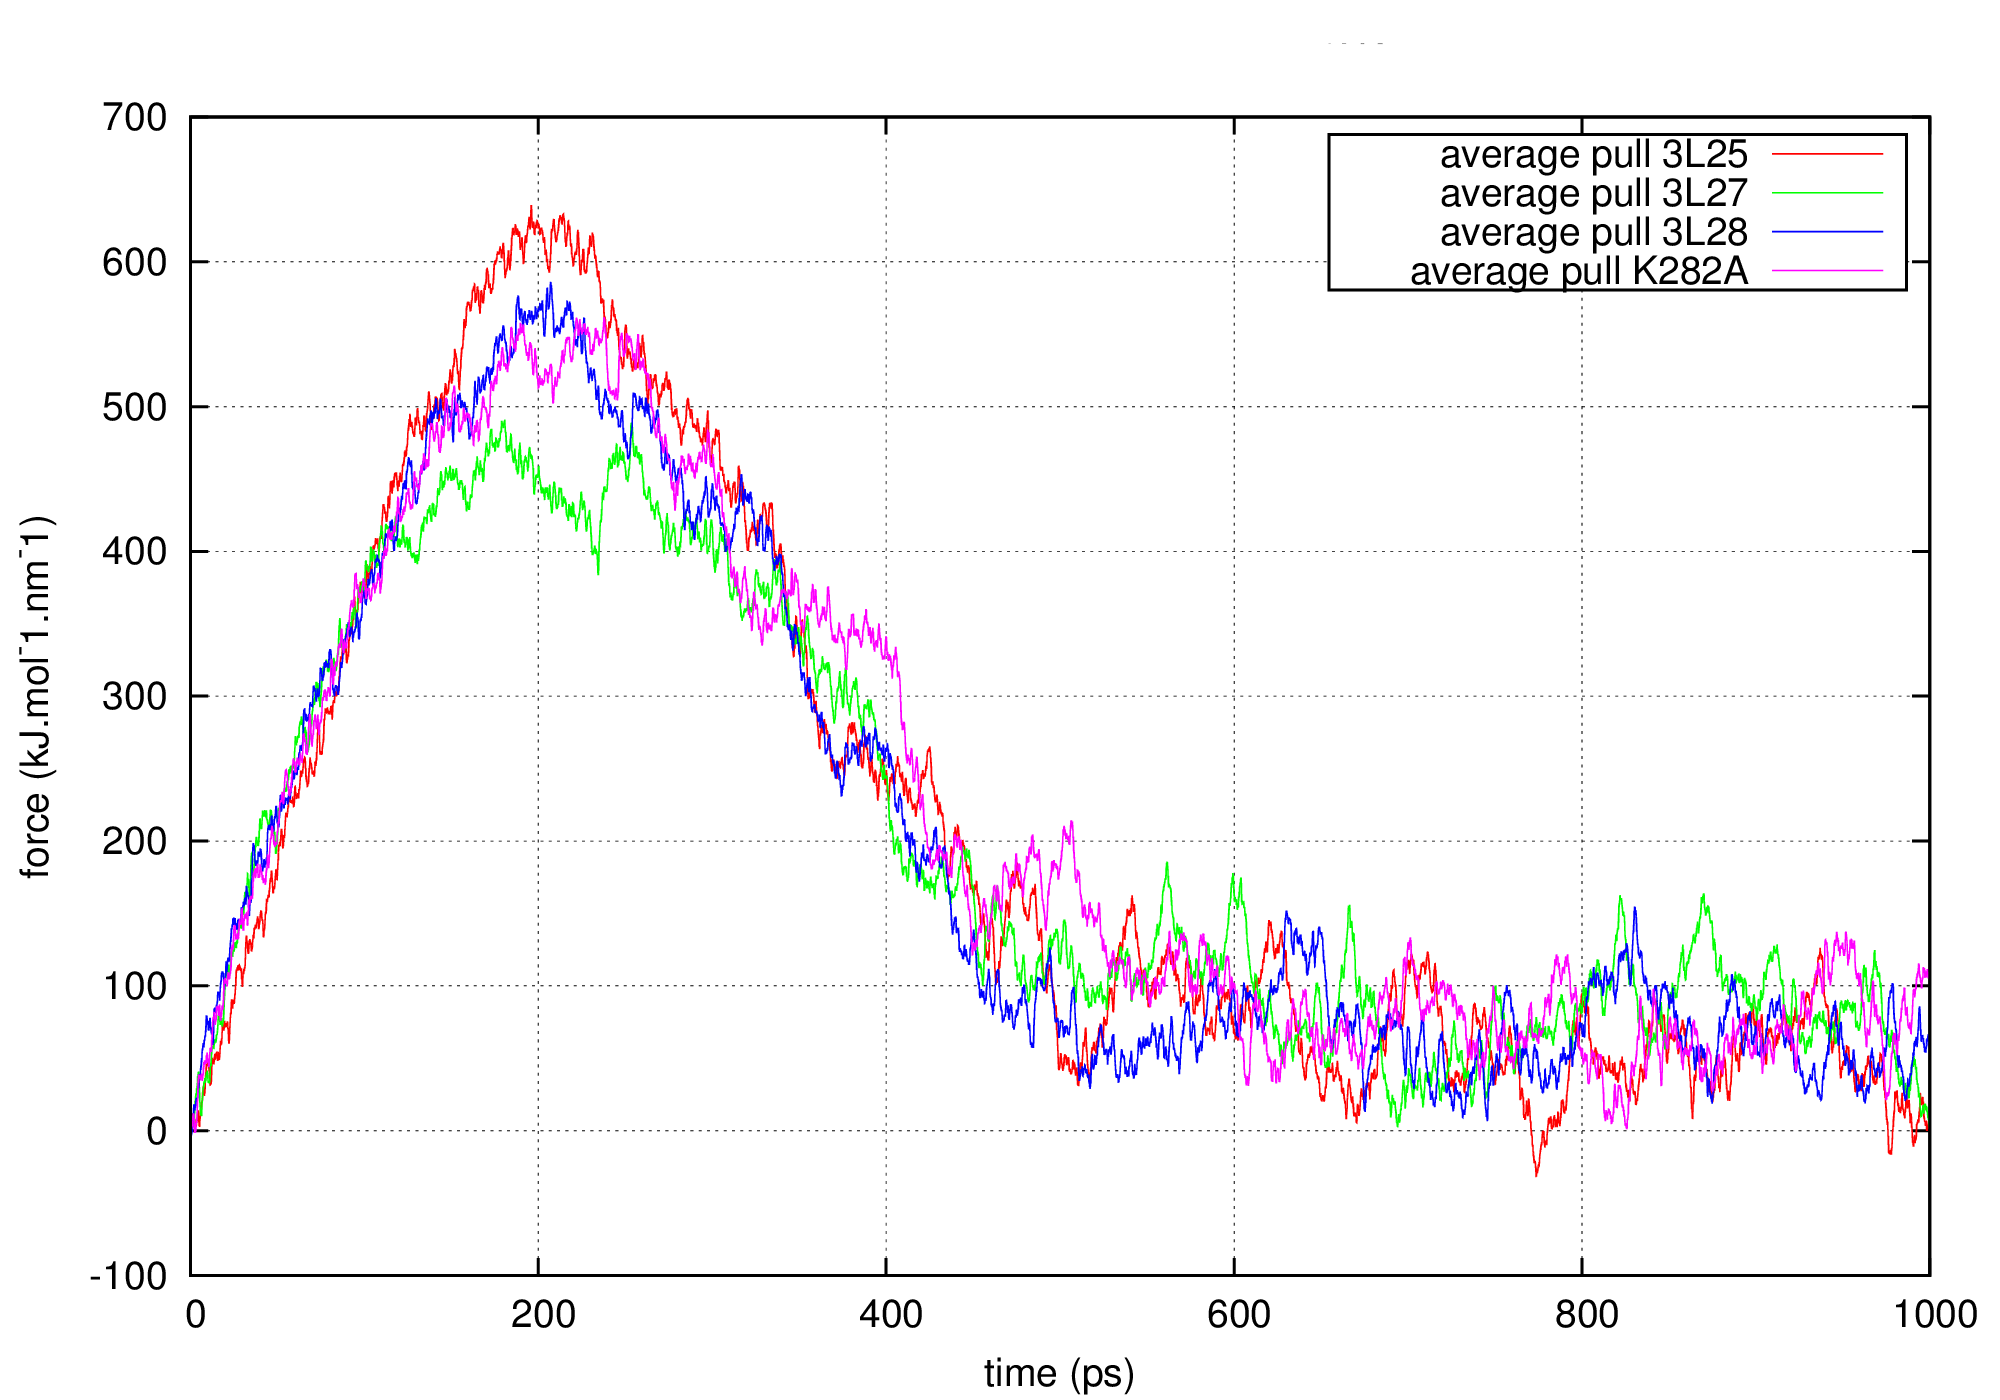
\includegraphics[width=0.7\textwidth,natwidth=610,natheight=642]{../pullf}
		\caption{Đường biểu diễn lực kéo trung bình theo thời gian giữa dsRNA và VP35 với phân tử không đột biến (3L25) và đột biến (3L27, 3L28, K282A)}
		\label{fig:pullf}
		\end{figure}
	\end{column}
	
	\begin{column}{0.5\textwidth}
	\begin{itemize}
	\item Lực kéo tối đa ứng với phân tử VP35 không đột biến (3L25) là lớn nhất.
	\item Lực kéo tối đa ứng với phân tử VP35 đột biến Arg312Ala (3L27) chênh lệch nhiều so với lực kéo phân tử không đột biến.
	\item Lực kéo tối đa ứng với phân tử VP35 đột biến Lys339Ala (3L28) và Lys282Ala thấp hơn so với cấu hình 3L25.
	\end{itemize}
	\end{column}
	\end{columns}
	\end{frame}


\subsection{Đột biến K282A}
	\begin{frame}{Đột biến K282A}
	\begin{itemize}
	\item Kết quả phân tích thế năng cho thấy Lys282 đóng góp nhiều vào tương tác dsRNA--VP35 [\ref{fig:potential}].
	\item Lys282 luôn tạo liên kết Hydro ở mức 100\% trong suốt thời gian VP35 vẫn còn tương tác với dsRNA [\ref{fig:hbond}].
	\item Lực kéo tối đa của Lys282Ala thấp hơn so với phân tử không đột biến (3L25), xấp xỉ lực kéo tối đa cho cấu hình đột biến Lys339Ala (3L28) [\ref{fig:pullf}].
	\end{itemize}
	\emph{Chưa có bằng chứng thực nghiệm vai trò của Lys282.}
	\end{frame}
	
\section{HƯỚNG PHÁT TRIỂN}
	\begin{frame}{Kết luận và Hướng phát triển}
		\begin{block}{Kết luận}
		\begin{itemize}
		\item Arg312 và Lys339 là hai vị trí amino acid có vai trò quan trọng đối với tương tác VP35--dsRNA. Điều phù hợp với thực nghiệm\cite{Leung2010}.
		\item Gợi ý vị trí amino acid Lys282 cũng đóng vai trò quan trọng trong tương tác VP35--dsRNA.
		\end{itemize}
		\end{block}
		\begin{block}{Hướng phát triển}
		\begin{itemize}
		\item Khảo sát phân tử VP35 đột biến Arg322Ala.
		\item Tiên đoán các phân tử có khả năng gắn vào khu vực tương tác dsRNA-VP35, gợi ý phân tử thuốc.
		\item Mô phỏng động học phân tử thời gian dài, tìm ra các amino acid đóng góp cho tương tác dsRNA-VP35.
		\end{itemize}
		\end{block}
	\end{frame}

%\subsection*{Tài liệu tham khảo}
\begin{frame}[allowframebreaks]{Tài liệu tham khảo}

\printbibliography

\end{frame}



\appendix
\section*{Appendix}
	\begin{frame}{Cực tiểu hoá năng lượng}
		\begin{figure}[h]
		\centering
		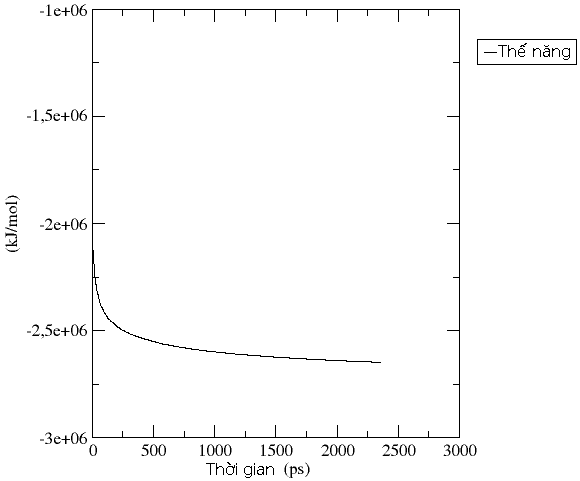
\includegraphics[height=0.35\textheight,natwidth=610,natheight=642]{../25energy}
		\caption{Đồ thị thế năng của hệ theo thời gian trong bước cực tiểu hoá năng lượng.}
		\label{fig:em}
		\end{figure}
		Giúp hệ hạt phân bố một cách ổn định trong không gian. Sau quá trình thế năng của hệ dưới $-2.5\times 10^{-6} kJ/mol$. Lực có giá trị lớn nhất là lực đặt lên nguyên tử thứ 210: $999 kJ.mol^{-1}.nm^{-1}$.
	\end{frame}
	
	\begin{frame}{Cân bằng chính tắc (NVT)}
		\begin{figure}[h]
		\centering
		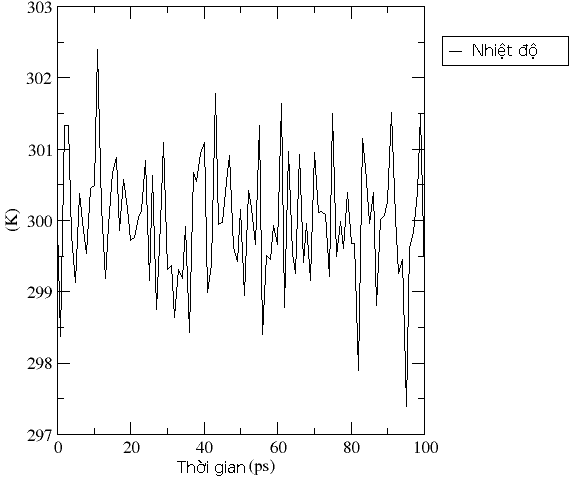
\includegraphics[height=0.35\textheight,natwidth=610,natheight=642]{../25temperature}
		\caption{Nhiệt độ trung bình của hệ theo thời gian trong bước cân bằng chính tắc (NVT)}
		\label{fig:nvt}
		\end{figure}
		Cố định chuỗi carbon chính, điều khiển nhiệt độ của hệ.
	\end{frame}
	\begin{frame}{Cân bằng đẳng nhiệt - đẳng tích (NPT)}
	\begin{columns}
	\begin{column}{0.5\textwidth}
		\begin{figure}
		\centering
		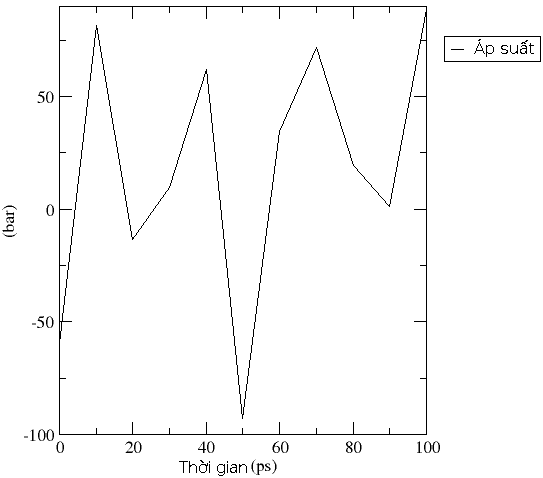
\includegraphics[height=0.3\textheight,natwidth=610,natheight=642]{../25pressure2}
		\caption{Áp suất của hệ theo thời gian trong bước cân bằng đẳng nhiệt - đẳng tích (NPT)}
		\label{fig:pressure}
		\end{figure}
		\begin{figure}
		\vspace{-30pt}
		\centering
		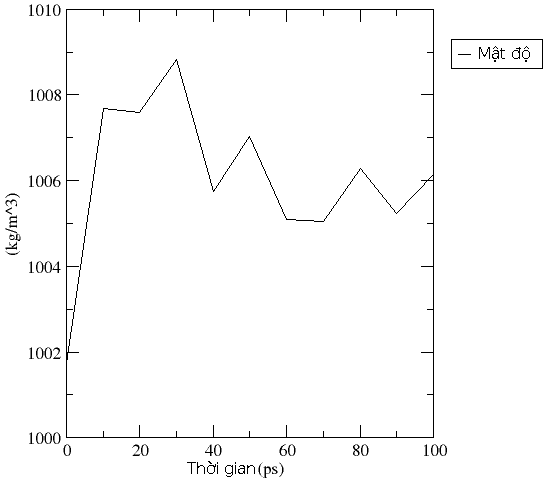
\includegraphics[height=0.3\textheight,natwidth=610,natheight=642]{../25density2}
		\caption{Mật độ của hệ theo thời gian trong bước cân bằng đẳng nhiệt - đẳng tích (NPT)}
		\label{fig:density}
		\end{figure}
	\end{column}
	
	\begin{column}{0.5\textwidth}
		\begin{itemize}
		\item Đồ thị \ref{fig:pressure} Lấy trung bình áp suất theo thời gian dài thì giá trị trung bình này lại không lớn.
		\item Đồ thị \ref{fig:density} cho thấy mật độ khối lượng của hệ vào khoảng $1006 kg/m^{3}$. Giá trị này tương đối phù hợp với mô hình nước TIP-4P\cite{Horn2004} đã được sử dụng.
		\end{itemize}
	\end{column}
	\end{columns}
	\end{frame}



%\beamertemplatebookbibitems
%\begin{thebibliography}{1}
%\bibitem{Author1990}A. Author. \newblock\emph{Handbook of Everything}.\newblock
%Some Press, 1990.\beamertemplatearticlebibitems
%
%\bibitem{Someone2002}S. Someone.\newblock On this and that\emph{.}
%\newblock\emph{Journal on This and That}. 2(1):50--100, 2000.\end{thebibliography}

\end{document}